\section{Layout}
\label{sec:ts-algorithm}
The layout algorithm to produce the positions of sets and events within them consists of four steps. First, the vertical ordering of sets is computed to ensure that two sets that share events are next to each other wherever possible. Then, sets are further divided into layers, and events are assigned to these layers according to their memberships. After that, the position and length of each event are computed, within the given display space. Finally, layers are compacted to remove any gaps between them, before their sizes are adjusted to yield a consistent level of detail across all sets.

\subsection{Sets Ordering}
\label{sec:set-ordering}
This step aims to maximize the number of events shared by neighboring sets, and can map to a graph path problem. Given a list of sets $S=\{s_1, s_2, \dotsc, s_n\}$, an undirected graph $G = (V,E)$ is created with each vertex $v_i$ representing a set $s_i \in S$. Two vertices $v_i$ and $v_j$ are connected if $s_i$ and $s_j$ share an event. The weight of edge $e_{ij}$ is the number of events shared by $s_i$ and $s_j$. Finding a set order with the maximum number of events shared by neighboring sets is equivalent to finding a path with the maximum weight connecting all vertices in $G$. This longest path problem is known to be NP-hard. However, the number of sets we plan to support is constrained by the number of colors that human can easily distinguish when they are shown together, which are only around 12 colors~\cite{Munzner2014}. Therefore, we decide to use a brute-force approach to find the optimal solution.

\subsection{Layer Layout}
% Requirements
This step positions all the events within a layer. Its input includes:
\begin{itemize}
	\item The events belonging to the layer with their \emph{label} and \emph{time} values.
	\item The maximum width and height of the layer.
\end{itemize}

The output includes locations of the input events within the constrained display area, optimized for the following criteria:
\begin{description}
	\item[Completeness] measures how much event labels are visible. More specifically, we define the \emph{completeness ratio} as:
	$\theta = \frac{\alpha \cdot |E_c| + \beta \cdot |E_t|}{|E|}$, where $|E_c|$ is the number of complete events, $|E_t|$ is the number of trimmed events, and $|E|$ is the number of all events. $\alpha$ and $\beta$ are the coefficients to indicate how strongly complete events and trimmed events contribute to the overall content richness of the layer, respectively. We practically set $\alpha=1$ and $\beta=0.5$.

	\item[Traceability] measures how easy it is to follow the events within a layer chronologically. Events happened close in time should have small changes in their row levels to maintain the reading flow. More specifically, we define the \emph{traceability ratio} as:
	$\gamma=\frac{\sum\limits_{i=1}^{|E|}(|l_{i+1} - l_i|)}{|E|-1}$	, where $|E|$ is the number of all events within the layer and $l_i$ is the row level of event $e_i$.
\end{description}

The horizontal position of an event is fixed by its time. The layout therefore decides on which row to position an event; i.e., vertical position, and the level of detail for its label.

\subsubsection{Completeness Layout}
This layout aims to display events with as much content as possible. Starting with an empty layer, events are processed chronologically. An event is located at the lowest possible row where it does not overlap with any other events. If such a row does not exist (because it reaches the height limit of the display), one of the earlier located events is trimmed to make space for that event. Among these events, the one with the least text being trimmed is selected. However, if the label space of that event is too short for a single word after trim, it will combine with the current event to form a new aggregated event labeled ``2 events''. Aggregated events cannot be trimmed, thus if a new event overlaps with them, it will be added into the existing aggregate. For example, a new event that overlaps with a ``2 events'' aggregated event will be grouped together producing the ``3 events'' aggregate.

The completeness layout maximizes the number of complete events $|E_c|$ and trimmed events $|E_t|$, thus yielding a maximum completeness ratio $\theta$. However, this layout does not optimize traceability because an event is located in the possibly lowest row disregarding the row level of its preceding event.

\subsubsection{Traceability Layout}
To improve traceability, this layout inserts a new event at the same row as its preceding event. If they overlap, the preceding event is trimmed to make space for the one currently added. We define the \emph{trim ratio} of an event as the ratio of the remaining text length to its original length. An event can only be trimmed if the resulting trim ratio is greater than a minimum threshold $t_{min}$, where $0\leq t_{min} \leq 1$. This value determines how much completeness can be traded for traceability. If the resulting trim ratio is smaller than $t_{min}$, the event moves up or down, up to $r_{max}$ rows on both sides, to find a satisfied row. $r_{max}$ decides how far, in terms of row level difference, an event can be from the preceding event, which essentially trades traceability for completeness. If no suitable row can be found within $\pm r_{max}$ rows, the currently adding event returns to the level of its preceding event and is then trimmed or aggregated with the preceding event as in the completeness layout.

\autoref{fig:traceability} shows an example of these two layouts. Both  run with linear time in terms of the number of events, because during the event insertion, the completeness layout checks up to a constant number -- the layer height -- of times, and the traceability layout checks at most ($2 \times r_{max}+1$) rows.

\begin{figure}
\centering
	\subcaptionbox{Completeness algorithm: $\theta=1$, \\$\gamma=5/3$.}{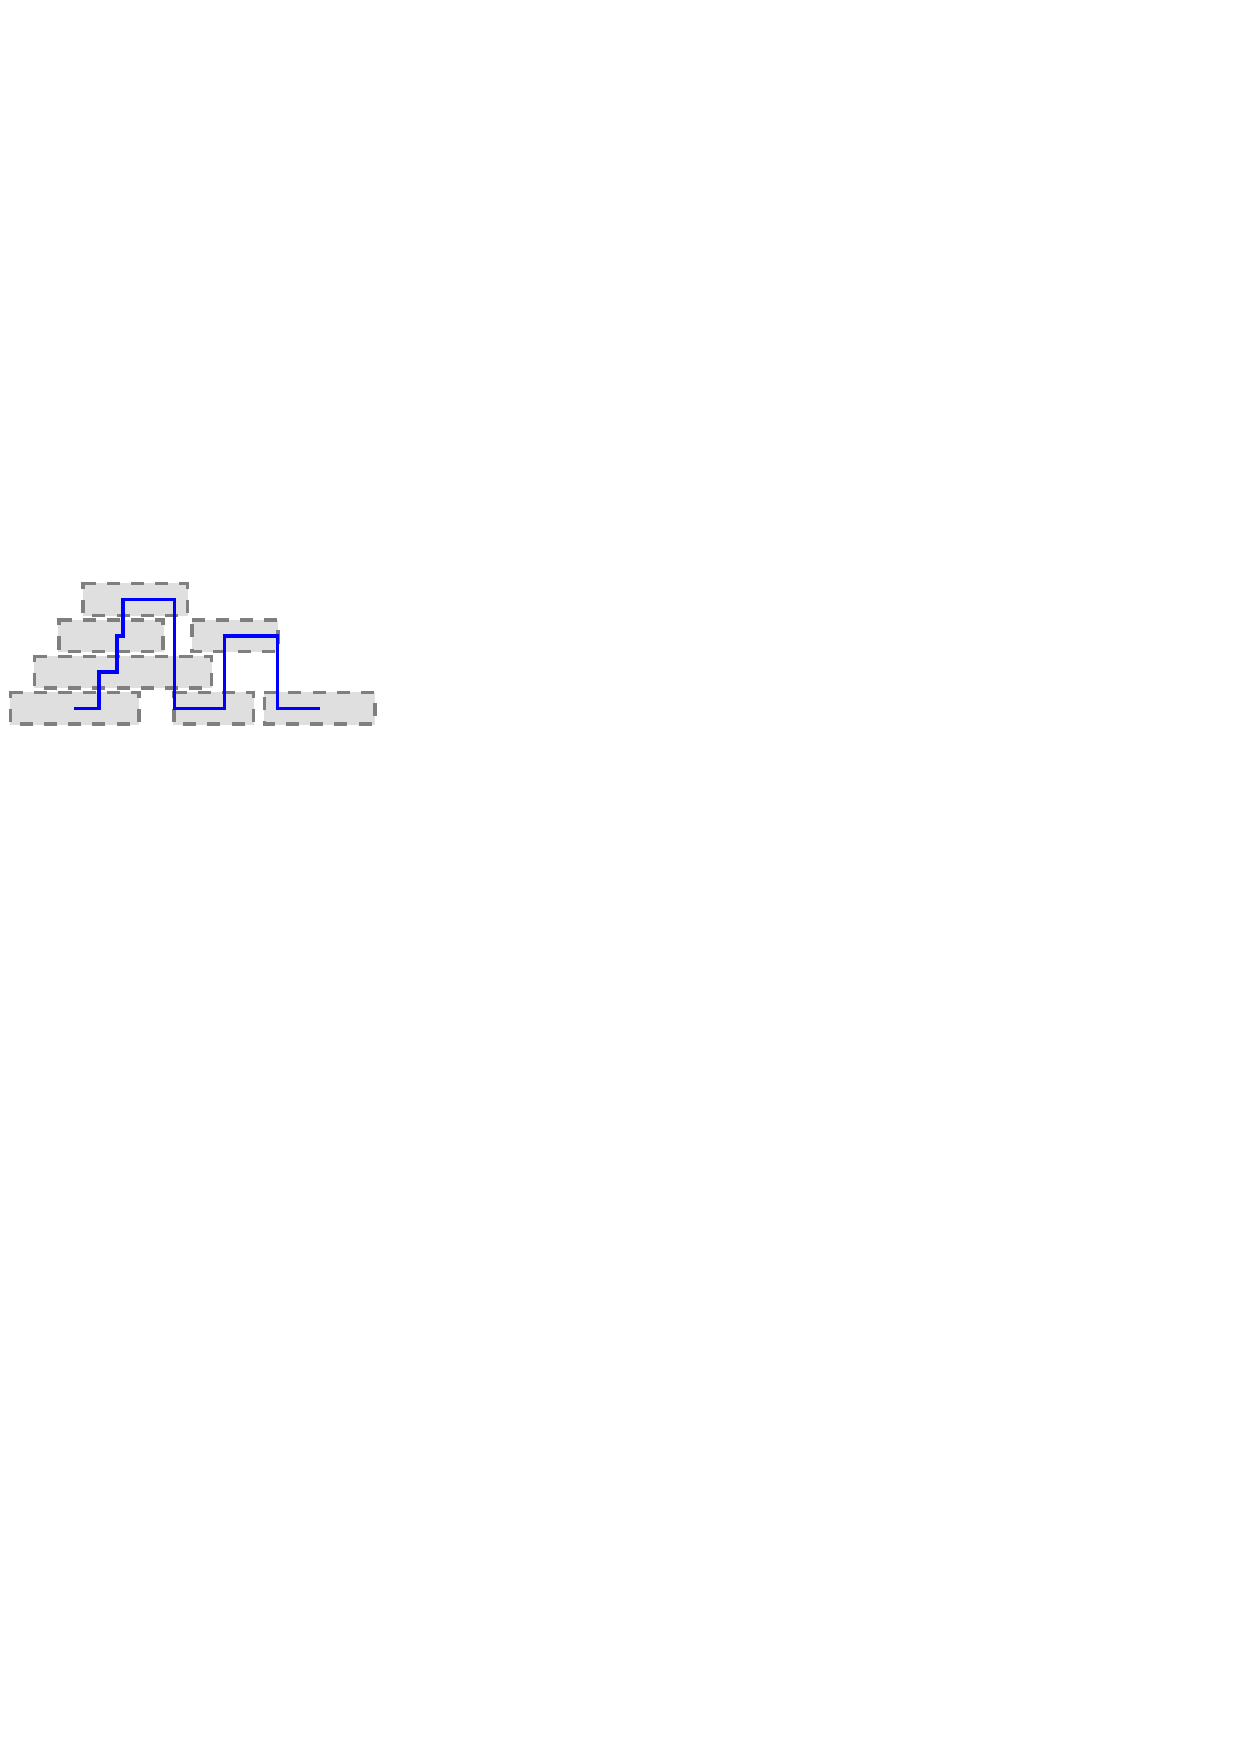
\includegraphics[width=.48\linewidth]{figure9a}}
	\hfill
	\subcaptionbox{Traceability algorithm with $t_{min}=0.5$ and  $r_{max}=1$: $\theta=6/7$, $\gamma=2/3$.}{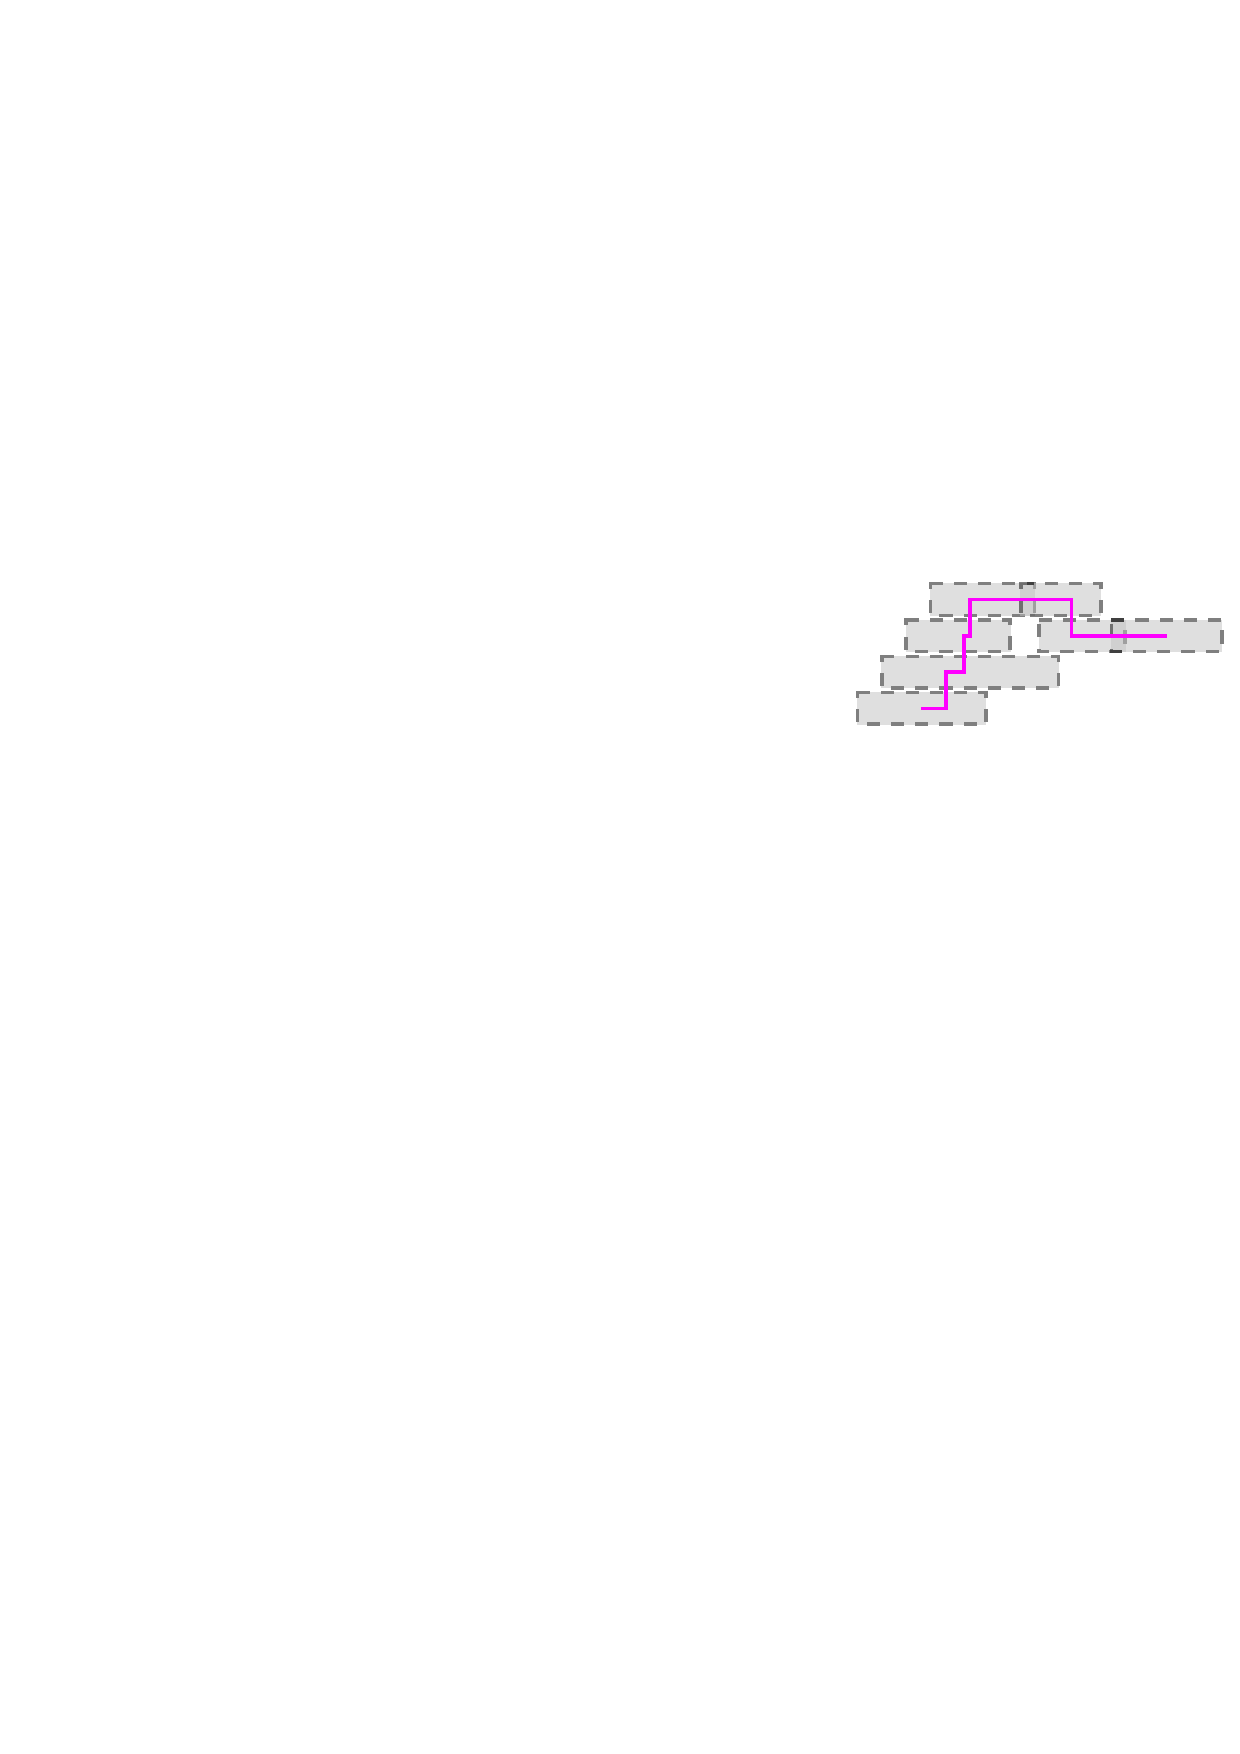
\includegraphics[width=.48\linewidth]{figure9b}}
\caption[Layer layouts]{Layer layouts. Each rectangle represents an event. The line connecting centers of rectangles illustrates the  traceability.}
\label{fig:traceability}
\end{figure}

\subsection{Compacting Layers}
\label{sub:compact}
After the layout of each layer is independently computed, layers are stacked together to produce a compact visualization. The two layer layouts require the layer height input as a maximum number of rows. Initially, that height is assigned proportionally to the number of events within each layer. However, some layers may not use all of their allocated space, resulting in gaps between layers that need to be filled. This includes moving two layers closer if there is a gap in between, or moving a layer into a newly created space if its set does not share events with any other sets. The freed space is assigned to the layer with the lowest completeness ratio $\theta$. Then, layouts of all layers are recomputed and compacted again. The process repeats until no more space can be saved. \autoref{fig:compacting} shows an example of compacting.

\begin{figure}
	\centering
	\subcaptionbox{Before: consumed height = 6 rows.}{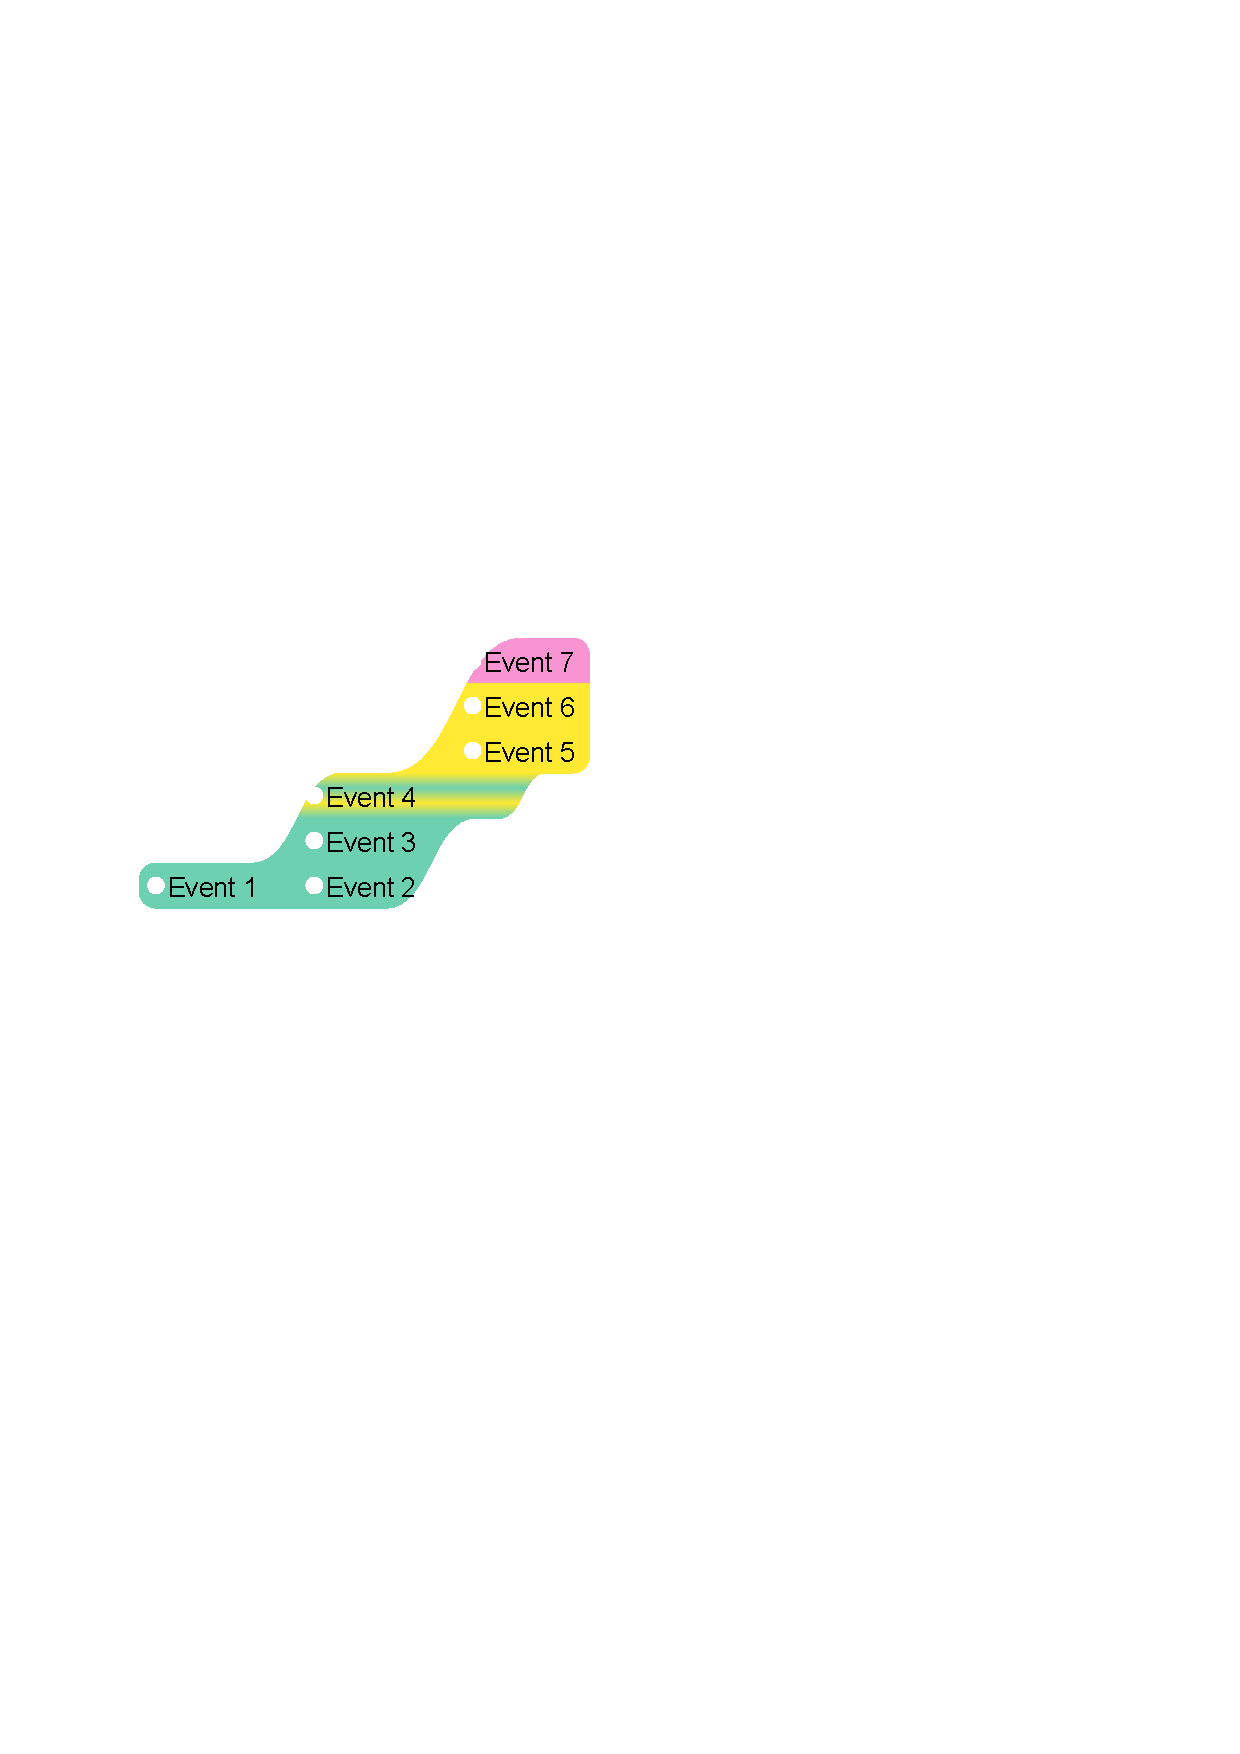
\includegraphics[width=.45\columnwidth]{figure10a}}
	\hfill
	\subcaptionbox{After: consumed height = 3 rows.}{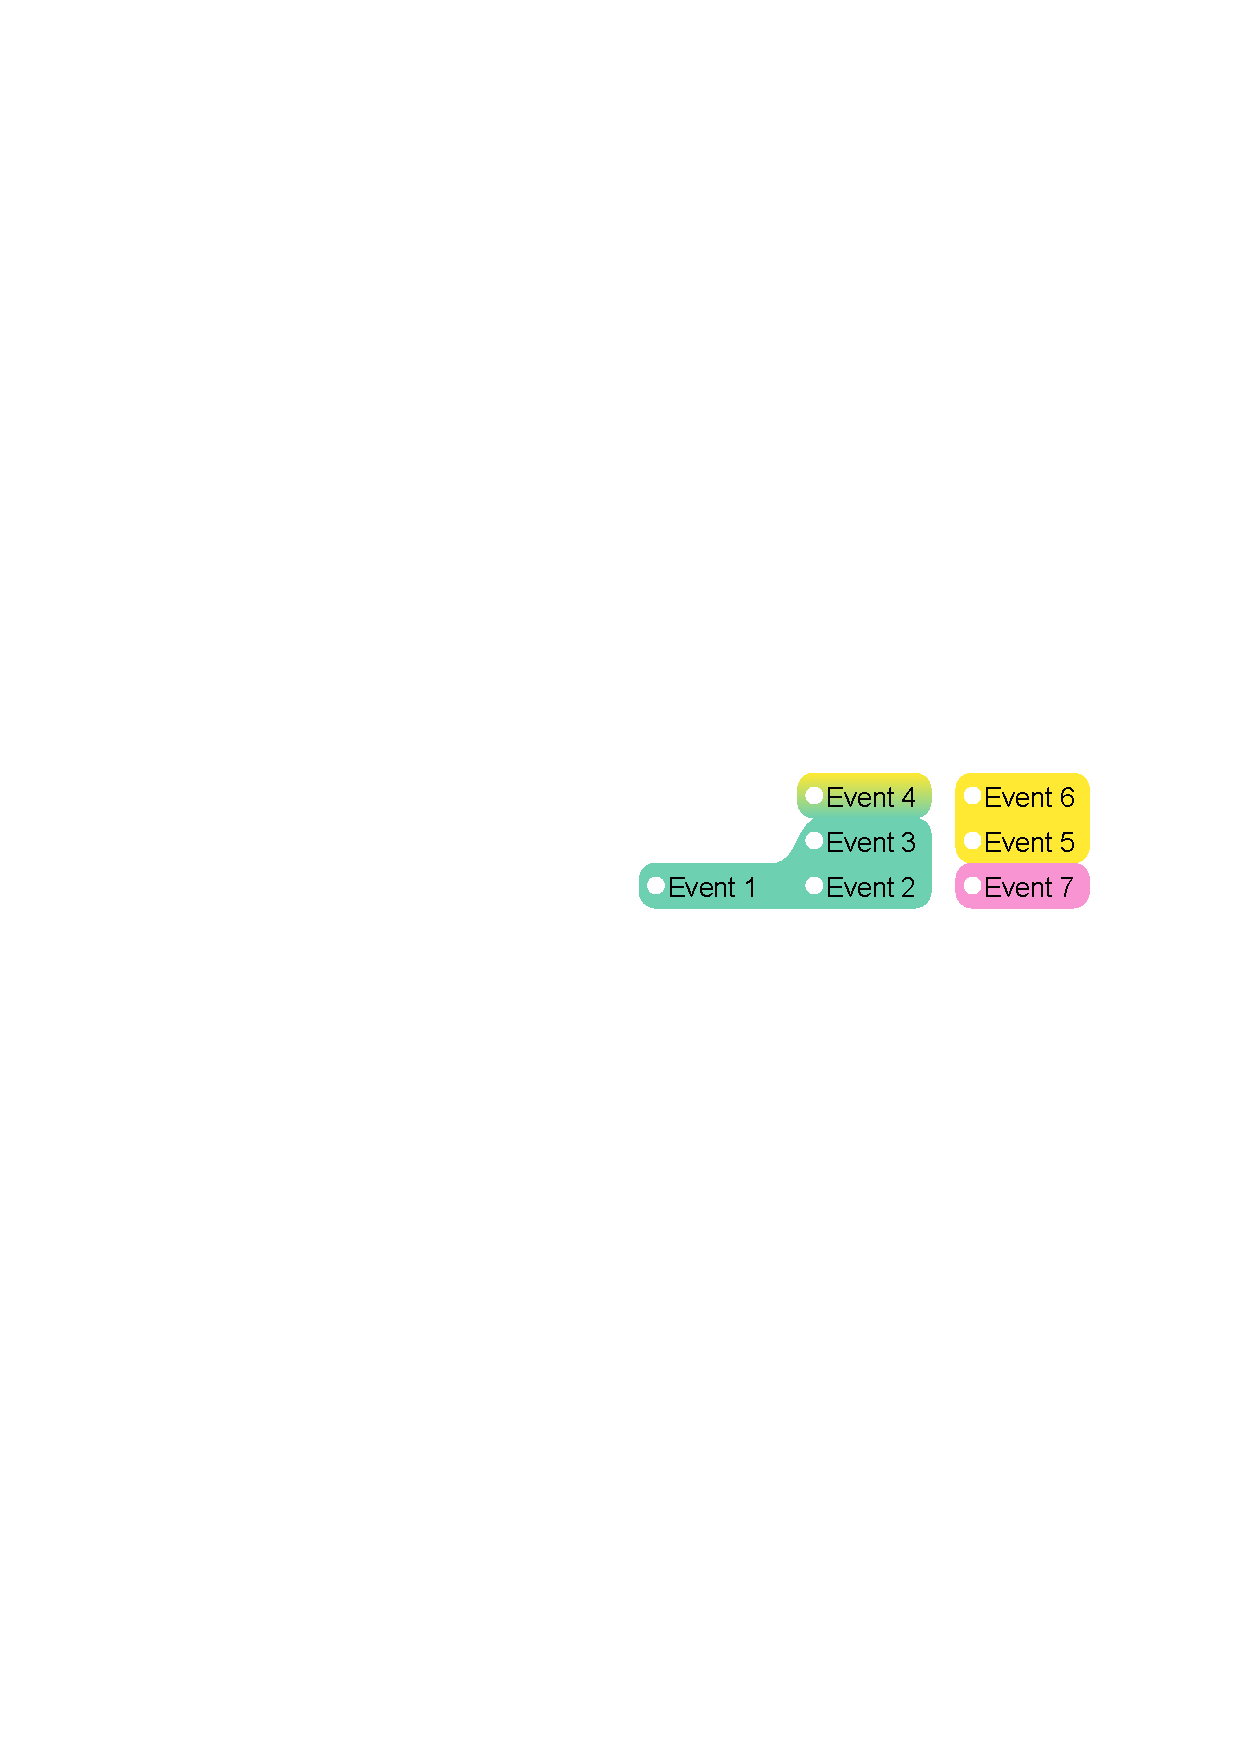
\includegraphics[width=.45\columnwidth]{figure10b}}
	\caption{Layers compacting.}
	\label{fig:compacting}
\end{figure}

\subsection{Balancing Layers}
This last step ensures that all layers have similar levels of detail; i.e., avoiding layers with many complete events and other layers with many aggregated events. This is achieved by minimizing the variance of completeness ratios of all layers,
$\frac{\sum\limits_{i=1}^{n}(\theta_i - \bar{\theta})^2} {n}$, where $n$ is the number of layers and $\bar{\theta}$ is the mean of all completeness ratios. A brute force approach tests all possible combinations of layer height $h_i$ such that $\sum\limits_{i=1}^{n}h_i=H$ for a minimum variance, where $H$ is the height of the display area. However, the number of combinations is an exponential of $n$. Instead, we apply a heuristic that relies on a simple observation that the completeness ratio increases with layer height. Therefore, the algorithm reduces the completeness ratio variance by iteratively transferring a row from the layer with the largest ratio to the layer with the smallest one, until the variance no longer decreases. \autoref{fig:balancing} shows an example of balancing.

\begin{figure}
	\centering
	\subcaptionbox{Before: $\theta_{green}=0.25$, $\theta_{yellow}=1$.}{\label{fig:balancing1}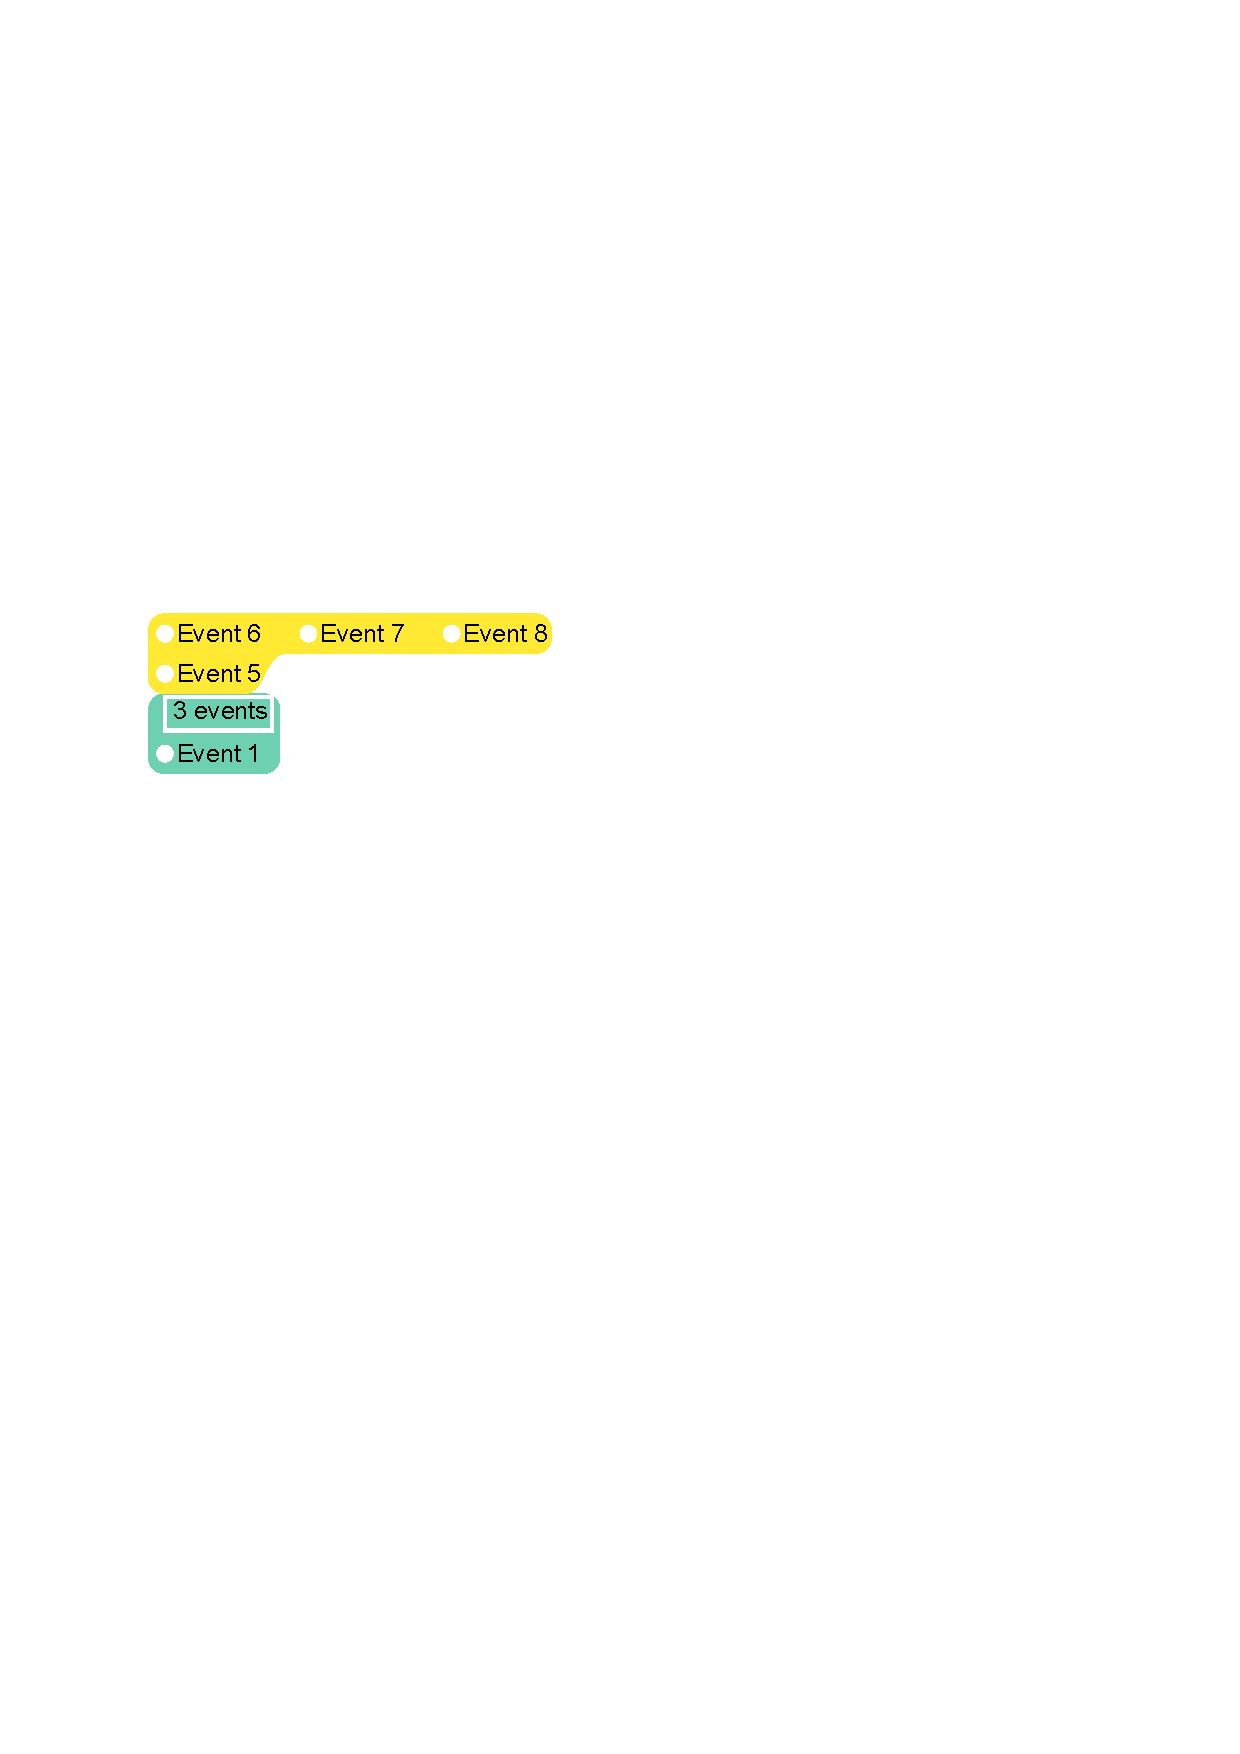
\includegraphics[width=.46\columnwidth]{figure11a}}
	\hfill
	\subcaptionbox{After: $\theta_{green}=\theta_{yellow}=0.5$.}{\label{fig:balancing2}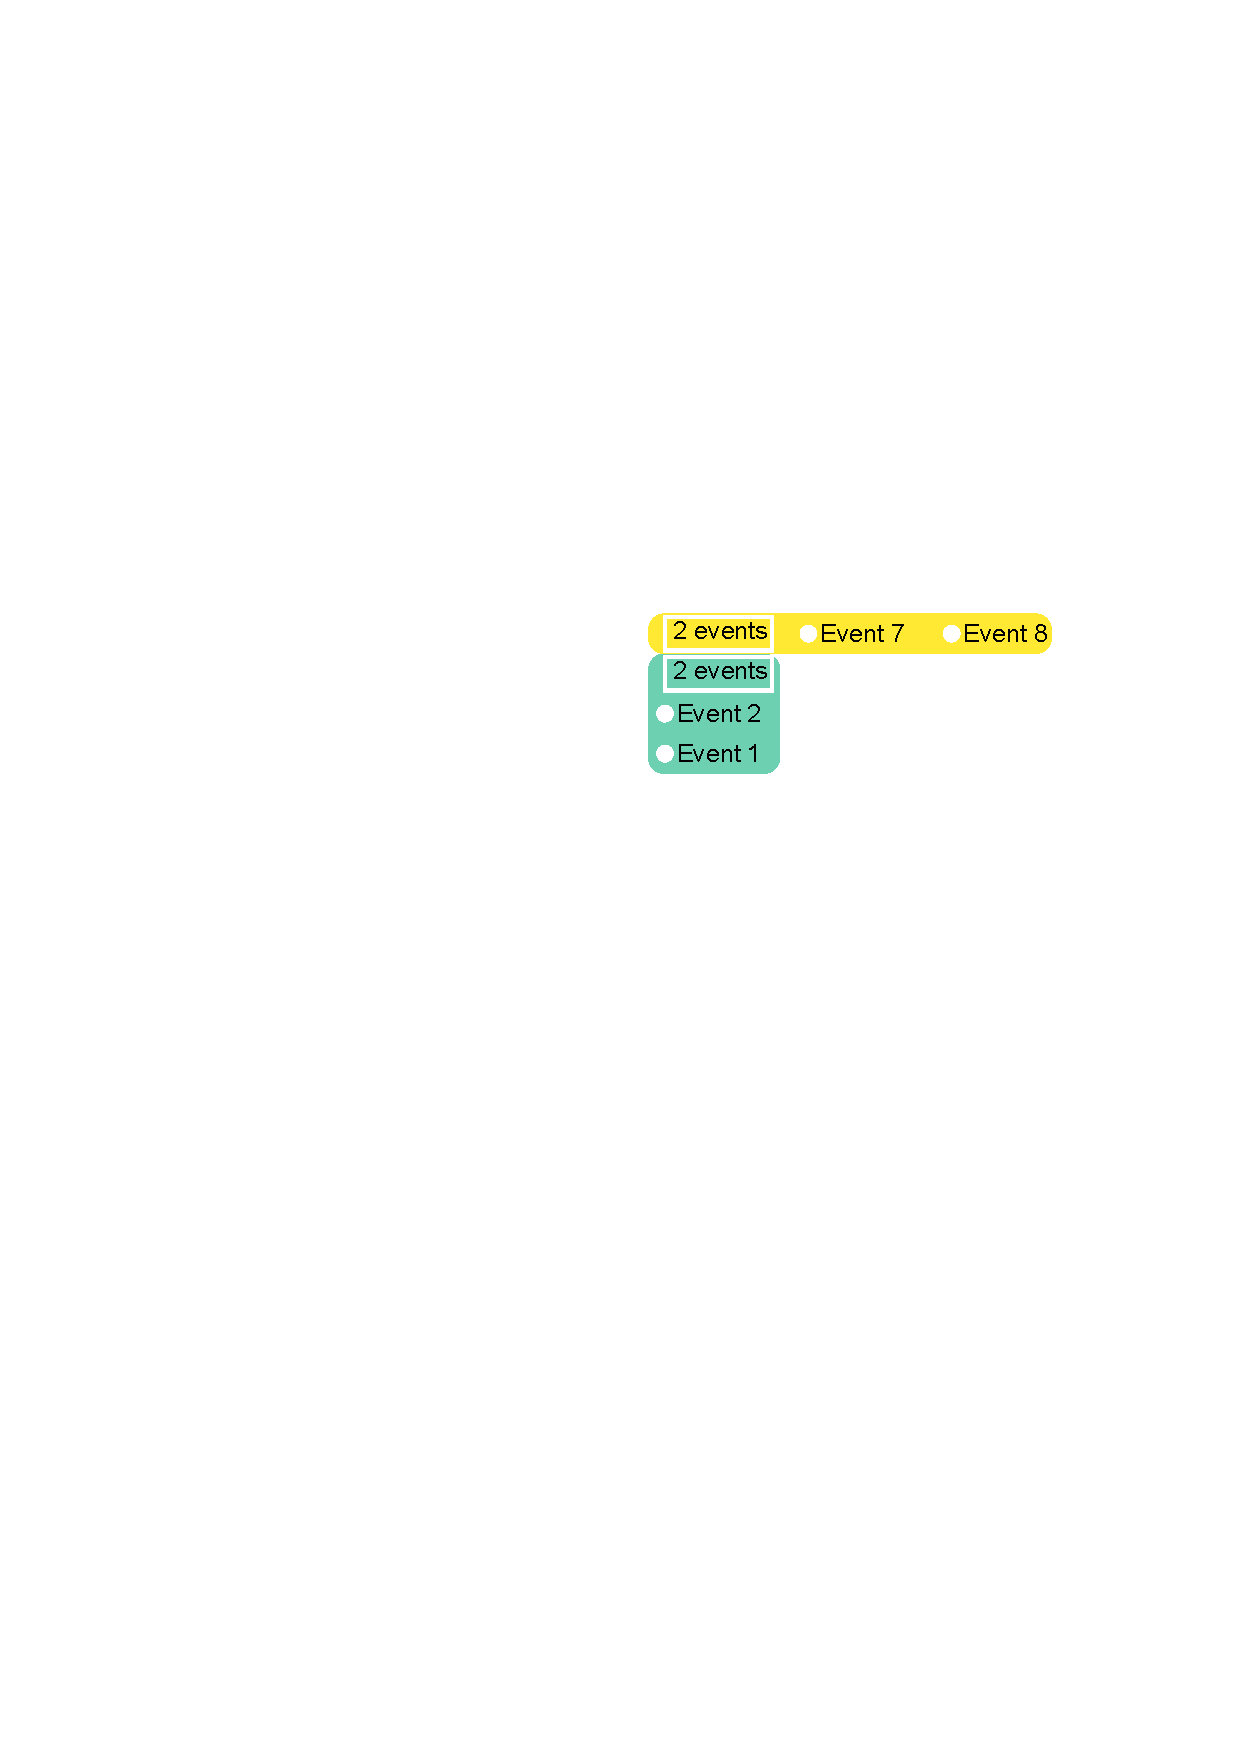
\includegraphics[width=.46\columnwidth]{figure11b}}
	\caption{Layers balancing.}
	\label{fig:balancing}
\end{figure}

\subsection{Scalability}
\label{sub:ts-scalability}
This section discusses the scalability of TimeSets: its capability, limitations and possible improvements. Aggregation enables TimeSets to visualize a large number of events. However, the visual representation of aggregated events is imperfect. For instance, two aggregates ``2 events'' and ``100 events'' are displayed exactly the same, except for the total number, whereas their sizes are largely different. We consider four options to address this issue as shown in \autoref{fig:ts-aggreate}.

\begin{figure}
	\centering
	\subcaptionbox{No encoding.\label{fig:aggregate-0}}{
		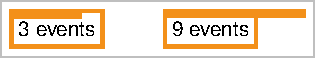
\includegraphics[width=.47\columnwidth]{figure12a}}
	\\
	\subcaptionbox{Each dot is an event indicating when it happens.\label{fig:aggregate-1}}{
		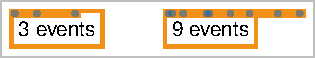
\includegraphics[width=.47\columnwidth]{figure12b}}
	\hfill
	\subcaptionbox{Scale with the width of the bounding rectangle.\label{fig:aggregate-2}}{
		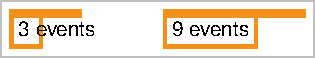
\includegraphics[width=.47\columnwidth]{figure12c}}
	\\
	\subcaptionbox{Color code the background of the bounding rectangle.\label{fig:aggregate-3}}{
		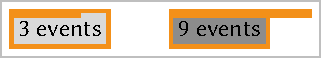
\includegraphics[width=.47\columnwidth]{figure12d}}
	\hfill
	\subcaptionbox{Scale with the font size of the label.\label{fig:aggregate-4}}{
		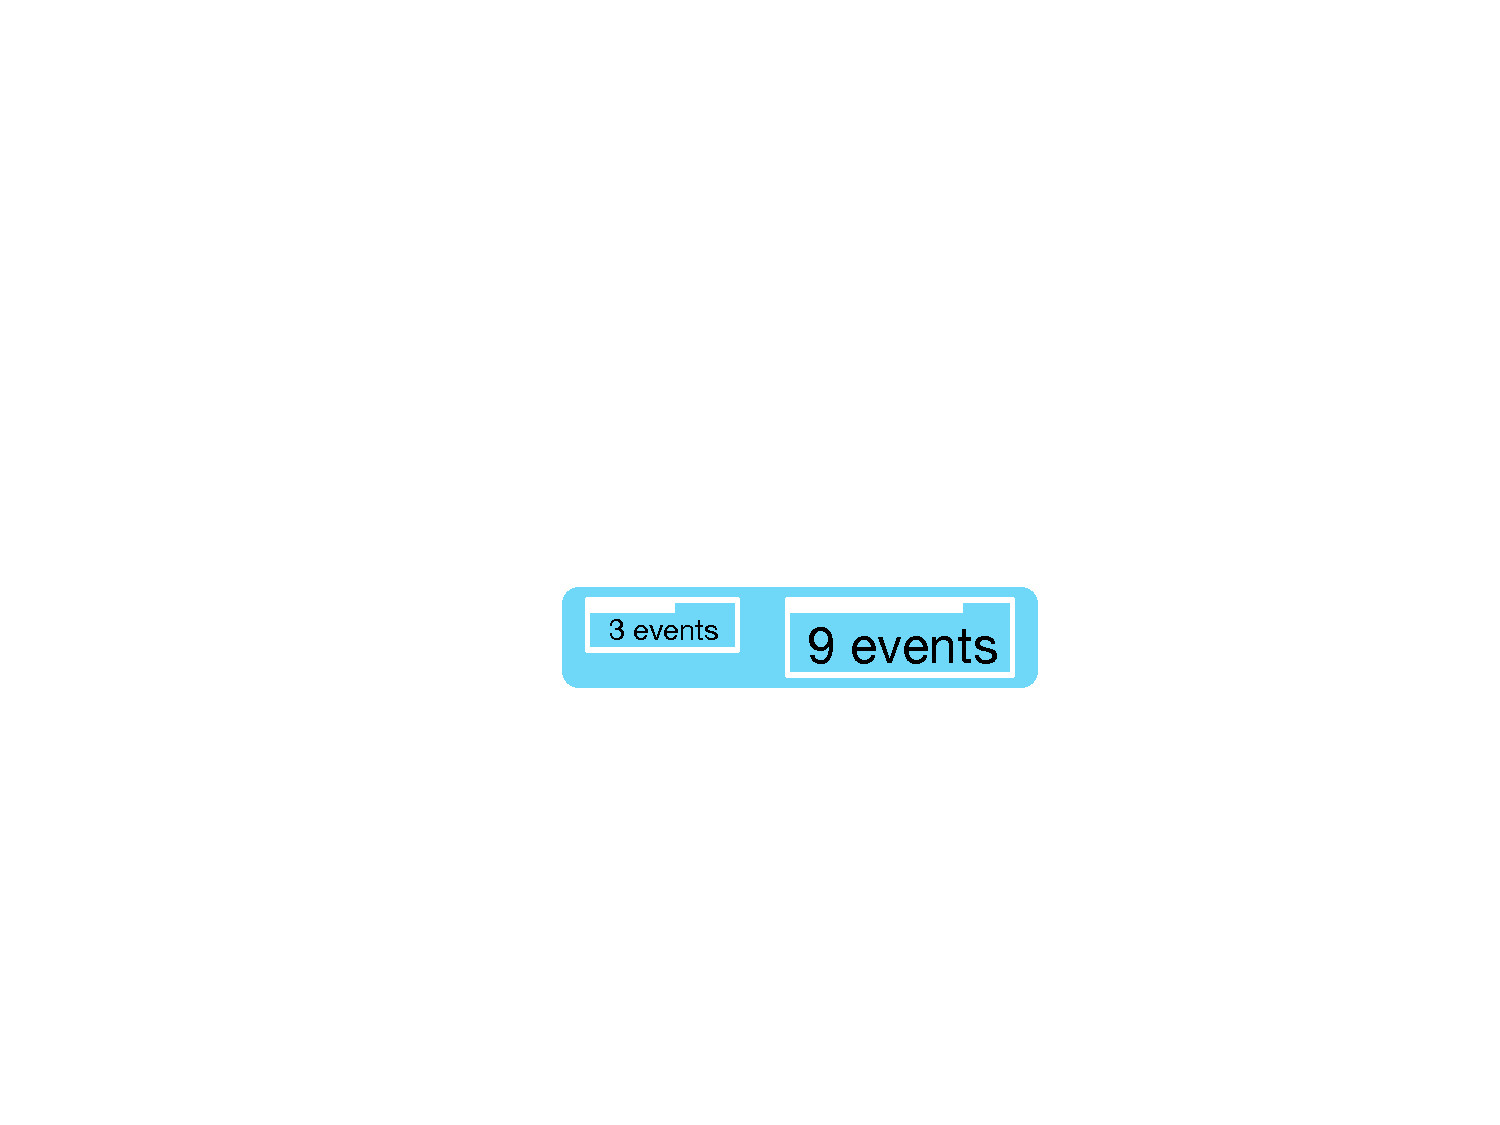
\includegraphics[width=.47\columnwidth]{figure12e}}
	\caption[Proposed visual representations of aggregates]{Proposed visual representations of aggregates emphasizing the number of its events.}
	\label{fig:ts-aggreate}
\end{figure}

The first option is to plot each individual event as a dot at when it happens (\autoref{fig:aggregate-1}). Besides providing a rough estimate of total count, this option also shows a temporal distribution of events. When events happen closely enough, their dots become overlapped, which makes it difficult to see the actual pattern.

Second, the width of the aggregate rectangle can be scaled to indicate the number of events (\autoref{fig:aggregate-2}). The full width of an aggregate rectangle is typically small as the length of its text ``$N$ events''. Therefore, the difference of aggregate widths could be subtle and difficult to observe from an overview.

Another option is to color code the background of the aggregate rectangle using luminance or intensity according to the number of events (\autoref{fig:aggregate-3}). However, when many aggregated events are displayed, their backgrounds could interfere with the set colors and distract users.

The last option we propose is to scale the font size of the label based on the number of events (\autoref{fig:aggregate-4}). Currently, each event is completely located in one single row with uniform height. Scaling the heights of aggregated events will affect the layout algorithm.

The existing layout is suitable for a small timeline with a few hundreds of events or a detailed view where individual events are of high importance. \autoref{fig:citations} shows TimeSets with a medium-sized publication dataset: 200 articles spanning 15 years. TimeSets relies on color to distinguish sets, therefore the number of sets it can support is constrained by the number of colors that a human can differentiate at the same time, which is about 12~\cite{Munzner2014}.